\documentclass[conference]{IEEEtran}
\usepackage{graphicx}
\usepackage{booktabs}
\usepackage{amsmath}
\usepackage{url}
\usepackage[hidelinks]{hyperref}
\usepackage{tikz}
\usetikzlibrary{arrows.meta,positioning,fit,backgrounds,calc}
\usepackage{listings}
\lstset{basicstyle=\ttfamily\scriptsize,columns=fullflexible,keepspaces=true,
        frame=single,framesep=3pt,breaklines=true}

% AUTO-GENERATED by tools/gds/collect_results.py: do not edit
\newcommand{\AsicTotalCells}{2266911}
\newcommand{\AsicBlocksDone}{11}
\newcommand{\AsicBlocksGds}{6}


\graphicspath{{figures/}}

\newcommand{\ember}{\textsc{Ember}}

\title{\ember{}: A From-Scratch GPU with an Integrated Int8 Tensor Unit \\
Architecture, Bit-Exact Verification, and Block-Level Physical Design on SkyWater 130\,nm}

\author{\IEEEauthorblockN{Toshal Kumbhar.}
\IEEEauthorblockA{Independent project RTL, software, and silicon flow by one person\\
\texttt{github.com/} \quad \today}
}

\begin{document}
\maketitle

\begin{abstract}
I present \ember{}, a GPU built completely from scratch without vendor IP,
HLS or a borrowed rasterizer. It runs a real 3D game loop, a complete Doom
level rasterized from the shareware IWAD, and a real neural network in RTL
simulation. I am also evaluating its logic blocks
through an open-source physical design flow to GDS-II on SkyWater 130\,nm.
The logical design contains a command processor with DMA and fences, a 512\,KB unified VRAM, a
four-lane IEEE-754 single-precision vector FPU, a geometry/setup engine, a
multi-cycle rasterizer with a Z-buffer, CLUT texturing and a full
read-modify-write output stage, a sprite blitter, vector video timing, and a
16$\times$16 int8 weight-stationary tensor unit, all behind a single
AXI4-Lite fabric. Every block is verified against an independent pure-Python
golden model and is \emph{bit-exact}: my cocotb suite passes
31/31 tests, including a CNN (LeNet-class) inference run at
98/100 = 98.0\% accuracy through the real RTL data path with trained int8
weights, and a 32-frame input-driven 3D game loop whose physics runs as a kernel
on the compute core. The worst measured frame takes 6.152\,ms, 18.6\% of a
30\,fps budget, using a 100\,MHz cycle-to-time conversion. These frequencies
are evaluation assumptions, not achieved post-layout operating frequencies.
Physical design targets twelve blocks through Yosys, OpenROAD, Magic and
KLayout. The generated results currently record \AsicBlocksDone{} completed
synthesis targets and \AsicBlocksGds{} exported block layouts with independently audited zero
routing violations and whole-layout Magic DRC errors. Remaining
blocks, LVS, timing closure, physical SRAM and chip integration are unfinished. I close with engineering lessons drawn from the debugging
process, which I consider the most transferable part of this project.
\end{abstract}

\begin{IEEEkeywords}
GPU architecture, rasterization, systolic array, int8 quantization, ASIC
implementation, sky130, open-source EDA, verification by golden model.
\end{IEEEkeywords}

\section{Introduction}

There are two ways to learn how a GPU works. The first is to read about it. The
second is to build one and watch it fail in ways no textbook describes. This
paper is about the second path.

\ember{} started from a deliberately awkward goal: build a GPU from scratch that
can run \emph{both} a basic AI workload and a basic game, on real hardware,
with an entirely open-source toolchain. ``From scratch'' is load-bearing here:
the rasterizer, the floating-point unit, the tensor array, the instruction set,
the assembler, the golden models, the C driver and the place-and-route are all
in this project. The only external pieces are a RISC-V soft core (NEORV32) as the
host, the sky130 process design kit, and the open EDA tools.

That constraint shaped everything. An FPU written from scratch means you must
come to terms with IEEE-754 subnormals, round-to-nearest-even, and what
``flush-to-zero'' does to your depth values at 2\,a.m. A rasterizer written from
scratch means you derive plane equations for $1/w$, colour, $u$, $v$ and depth,
and then discover that your interpolator is off by one bit at the right edge of
the screen. A tensor unit written from scratch means you learn why weight-stationary
systolic arrays are shaped the way they are, and why the tricky part is not the
multiplier array but the address generator feeding it.

The result is a small but genuine GPU. It is not fast and it does not pretend to
be: its rasterizer uses multiple cycles per pixel and its tensor array is
streaming-limited. The RTL demos are verified; physical implementation is a
separate, incomplete workstream. I
also find the ``wrong'' parts of the story more useful to other engineers than
the successful parts, so I document them explicitly in
Section~\ref{sec:lessons}.

\subsection*{Contributions}
\begin{itemize}
  \item \textbf{A complete, verified GPU architecture} (Section~\ref{sec:arch}):
        command processor, unified memory, geometry engine, rasterizer with
        Z-buffer and texturing, blitter, display, compute core and tensor unit,
        with a documented register map and command queue format.
  \item \textbf{A 32-bit SIMT-style ISA and assembler} (Section~\ref{sec:core})
        used to write real kernels, including a fixed-point game-physics kernel
        that runs the demo's per-frame integration on the chip itself.
  \item \textbf{An int8 tensor unit that actually infers} (Section~\ref{sec:tu}):
        a LeNet-class CNN trained in pure Python, quantized, and executed
        through the RTL at 98.0\% accuracy, bit-identical to a software mirror.
  \item \textbf{A real game level through the same pipeline} (Section~\ref{sec:doom}):
        10{,}774 textured triangles built from Doom's own BSP geometry, composed
        wall textures, flats and light tables, rasterized by the RTL
        bit-exactly against the golden model (76{,}800 of 76{,}800 pixels).
  \item \textbf{A verification methodology that scales down} (Section~\ref{sec:verify}):
        one golden model per block, differential testing, structural assertions
        for demos where no golden pixel exists, and a 31/31 suite.
  \item \textbf{Block-level ASIC flow evaluation} (Section~\ref{sec:asic}):
        measured synthesis and layout results with explicit completion status,
        independent exported-GDS checks and unresolved implementation limits.
  \item \textbf{An honest lessons section} (Section~\ref{sec:lessons}) covering
        the bugs that a textbook would not warn you about.
\end{itemize}

\section{Related Work}
\label{sec:related}

\textbf{Open-source GPUs.} RasterIX, voodoo-fpga and Polyphony demonstrate
hardware rasterization on FPGAs; Project F provides well-documented FPGA
graphics building blocks. They concentrate on the graphics pipe. \textbf{GPGPU
research} includes MIAOW (an open AMD GCN RTL implementation), Nyuzi and Vortex,
which are RISC-V GPGPU designs with real compiler stacks. These target much
larger platforms than this design. \textbf{Tensor hardware} spans Google's TPU v1
(a 256$\times$256 int8 systolic array) down to Gemmini and many FPGA CNN
accelerators; the weight-stationary dataflow I use is the classic
Kung--Leiserson arrangement that the TPU paper brought back into fashion.
\textbf{Verification practice} in the open-source world is dominated by
cocotb plus Verilator; I lean heavily on that pairing and on the discipline of
writing an independent model in a different language from the RTL.

What distinguishes \ember{} is not any single block. It is that the graphics
pipe, the tensor pipe, the compute cores, the host interface and the physical
implementation all exist in one coherent design, verified end-to-end by
software that also runs on the chip's own instruction set.

\section{Architecture}
\label{sec:arch}

\begin{figure*}[t]
\centering
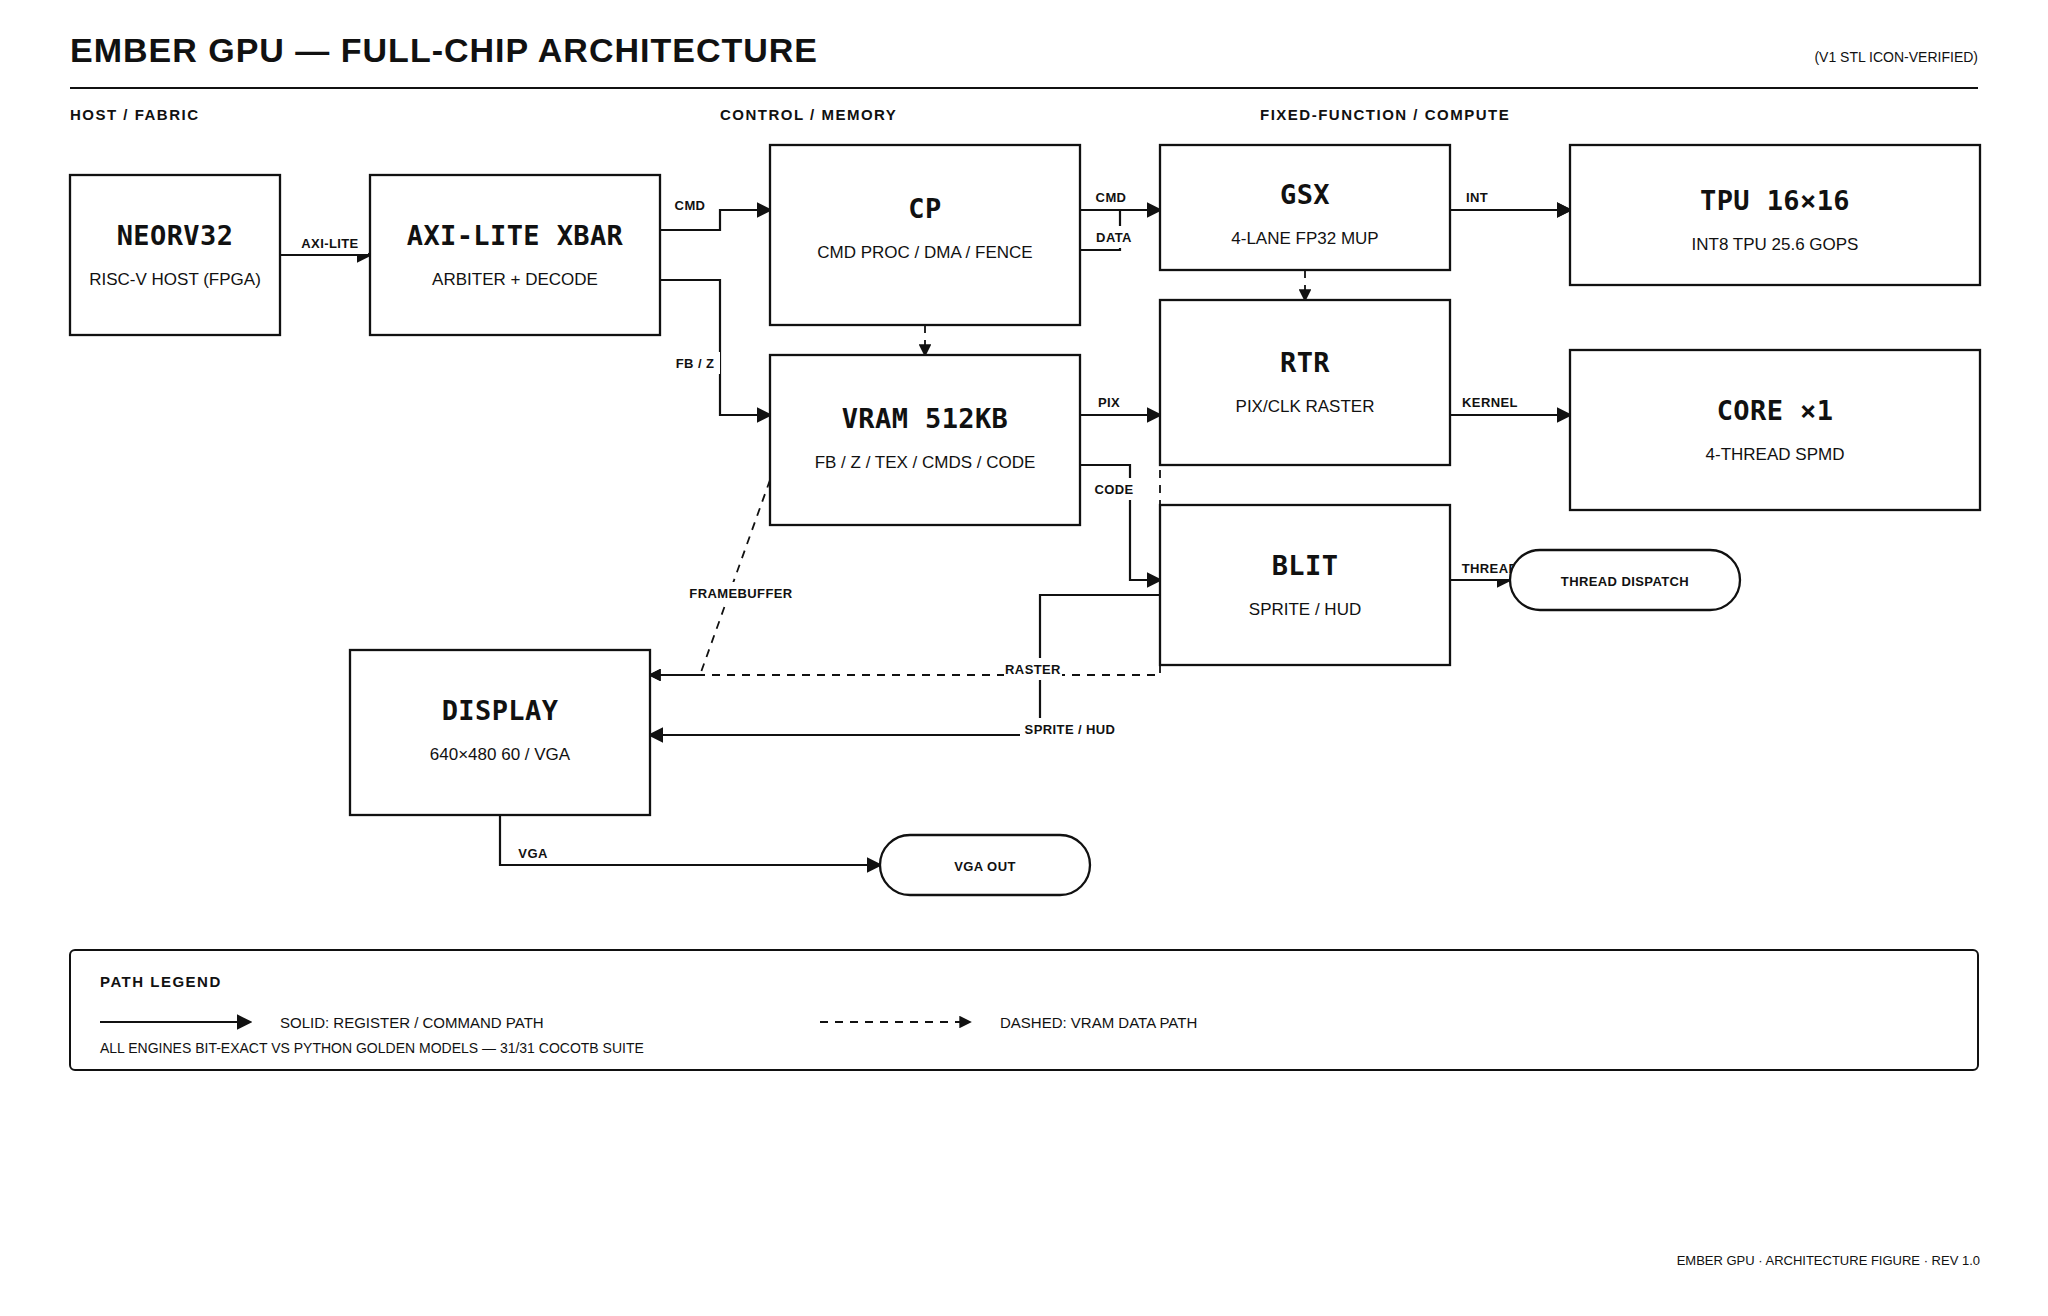
\includegraphics[width=0.86\textwidth]{architecture.png}
\caption{The \ember{} chip. Solid arrows are register/command paths; dashed
arrows are VRAM data paths. The host drives a flat AXI4-Lite port; the
crossbar decodes to the command processor and VRAM. Every accelerator is
started by a register write from the CP and reports completion through
\texttt{STATUS}. The rasterizer, blitter and display own dedicated VRAM pixel
ports, reducing fabric contention during multi-cycle rasterization.}
\label{fig:arch}
\end{figure*}

Figure~\ref{fig:arch} shows the chip. There is one memory system and two
accelerators: a graphics pipe and a tensor pipe.

\subsection{Command Processor and Memory}

The host never talks to an accelerator directly. It talks to the CP, which owns
a small register file, a 64-entry upload FIFO, an 8-entry readback FIFO, a DMA
engine, a completion counter used as a fence, and one ``kick'' register per
accelerator:

\begin{center}
\resizebox{\columnwidth}{!}{%
\begin{tabular}{@{}ll@{}}
\toprule
Register & Function \\
\midrule
\texttt{STATUS} & dma/rtr/blit/cp/core/tu busy + readback level \\
\texttt{FIFOD} & write = push upload word, read = pop readback word \\
\texttt{DMA\_SRC/DST/LEN} & FIFO$\to$VRAM and VRAM$\to$FIFO transfers \\
\texttt{RTR\_KICK} & start a triangle sweep from the command queue \\
\texttt{BLIT\_*} & rectangle source/destination/size/flags \\
\texttt{GSX\_*} & matrix, vertex stream, colour, configuration, go \\
\texttt{CORE\_CODE/NBLK/KICK} & load and launch a kernel \\
\texttt{TU\_*} & operand bases, dimensions, quantization, go \\
\bottomrule
\end{tabular}}
\end{center}

VRAM is 512\,KB and holds everything: the framebuffer at \texttt{0x000000}, the
Z-buffer at \texttt{0x025800}, texture pages at \texttt{0x04B000}, the RTR
command queue at \texttt{0x05B000} and kernel code at \texttt{0x05B400}. That
single flat map is deliberately simple: any debug tool, any golden model and any
driver can address any pixel with one 32-bit number. The map went through a
painful revision early on, the original layout had the command buffer
overrun the end of memory and wrap into the framebuffer, and the fix taught
me to size every region against the fabric's real capacity rather than its
nominal one.

\subsection{Interconnect}

A 2$\times$2 AXI4-Lite crossbar connects two masters (host and CP-DMA) to two
slaves (CP registers and VRAM), with round-robin arbitration and a lock-based
forwarding scheme so that a read-modify-write sequence cannot be split by the
other master. The rasterizer, blitter and display bypass the fabric on dedicated
pixel ports, reducing contention with host accesses during rendering.

\section{Compute Core and Instruction Set}
\label{sec:core}

The compute core is a four-thread SPMD machine executing a 32-bit
\textsc{Ember-ISA v2}. Sixteen general-purpose registers plus three read-only
ones (\texttt{\%blockIdx}, \texttt{\%blockDim}, \texttt{\%threadIdx}) are
provided per thread; each thread has its own program counter and its own
one-word instruction buffer. Instructions fall into four classes:

\begin{itemize}
  \item \textbf{Integer ALU:} \texttt{ADD}, \texttt{SUB}, \texttt{MUL},
        \texttt{DIV}, \texttt{MIN}, \texttt{MAX}, \texttt{AND}, \texttt{OR},
        \texttt{XOR}, \texttt{SHL}, \texttt{SHR}, \texttt{CMP}.
  \item \textbf{Floating point:} \texttt{FADD}, \texttt{FSUB}, \texttt{FMUL},
        \texttt{FDIV}, issued to the vector FPU.
  \item \textbf{Memory:} \texttt{LD}/\texttt{ST} through one port,
        \texttt{LDS}/\texttt{STS} to per-core shared memory with
        \texttt{ATOMIC\_ADD} and \texttt{ATOMIC\_MAX}.
  \item \textbf{Control:} \texttt{BRNZP}, \texttt{JAL}, \texttt{JR},
        \texttt{CALL}, \texttt{RET} and the block barrier \texttt{BAR}.
\end{itemize}

Two design decisions in this core are worth calling out because they were
forced by deadlocks rather than chosen for elegance. First, the fetch channel
and the data channel are \emph{separate VRAM ports}: with one shared read port,
a thread waiting on a load holds the instruction buffer while the fetch that
would unblock it cannot be issued, a circular wait that hangs the core
forever. Second, instruction buffers are \emph{per thread}: with a single shared
buffer, thread~0 reaches the barrier, its next word wedges the buffer, and
threads 1--3 never arrive, the classic broken barrier. Both fixes are
invisible in a tiny test and fatal in a real one.

Kernels are written in assembly and assembled by my two-pass assembler, which
supports labels, \texttt{.word}/\texttt{.string}/\texttt{.org} directives and
pc-relative branches. Real kernels in the repository include matrix multiply,
2$\times$2 max-pool with a signed-byte trick, and the game-state kernel below.

\subsection{The game-state kernel: a game loop on the chip}

The most satisfying moment in this project was moving the camera physics out of
the testbench and onto the core. \texttt{gamestate.asm} (112 words) runs a
Q16.16 fixed-point loop, once per frame, on thread~0:

\begin{lstlisting}
; in = input word (bit0 = forward, bit1 = left, bit2 = right)
vel += in*ACC          ; accelerate, ACC = 1638 (0.025/frame^2)
f   = |vel| >> 4       ; friction: 1/16 of speed per frame
vel -= sign(vel)*f     ; signed decay, symmetric
vel  = clamp(vel, -VMAX, +VMAX)
pos += vel             ; integrate
pos  = clamp(pos, x in [-2,2], z in [0,1])
out  = f2q(pos)        ; exact Q16 -> IEEE-754 fp32 bit pattern
\end{lstlisting}

The kernel then writes the camera state back to VRAM and echoes a cookie so the
host can confirm completion, and precomputes the one MVP word it can compute
exactly (a pure Q16 add), leaving the other to the host because it needs a
37-bit product. The physics is bit-exact against the Python mirror on all 32
frames of the demo, meaning the camera walk you see in
Figure~\ref{fig:input} is the result of instructions executed by the GPU.

\section{Graphics Pipeline}
\label{sec:gfx}

\subsection{GSX: geometry and setup}

The geometry engine contains a four-lane IEEE-754 single-precision FPU built
from scratch: round-to-nearest-even, flush-to-zero, correct NaN/Inf handling and
a fixed six-cycle latency (issue on cycle $N$, result at $N+5$), fixed
latency rather than a busy/wait protocol, because polling a busy flag raced the
lane state machine and occasionally read a zero result.

GSX loads a 4$\times$4 MVP matrix, streams vertices five words at a time
($x,y,z,u,v$), transforms them four at a time, divides $x/w$, $y/w$, $z/w$ in
one parallel FPU pass, culls triangles with $w \le 0$, converts to Q10.22 and to
a 16-bit depth, and emits 19-word command packets into the command queue in
VRAM. The pipeline is deliberately fixed-function: this is a PS1-class machine,
and a machine that draws correctly is worth more here
than a programmable shader that draws slowly.

\subsection{RTR: rasterize, texture, output}

Setup uses Cramer's rule on the triangle's edge functions to produce plane
coefficients for $1/w$, red, green, blue, $z$, $u$ and $v$; the $1/w$ plane is
constant in this revision, which is why texturing is affine. The scan unit then
walks the bounding box through multi-cycle coverage test, plane
evaluation, a divide for perspective-correct interpolation, Z-test (less-than),
CLUT texture lookup, and a full read-modify-write output stage: clamping,
colour mapping, optional 50\% blend, $\pm1$ ordered dither, and RGB565 packing
into a byte-packed framebuffer.

\begin{figure}[t]
\centering
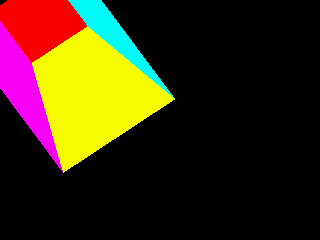
\includegraphics[width=\columnwidth]{cube_rtl.png}
\caption{A spinning cube rendered by the RTL rasterizer, per-pixel bit-exact
against the golden model. The gradient background comes from the same
fixed-function pipeline.}
\label{fig:cube}
\end{figure}

Triangle commands are fetched from a zero-terminated 19-word-per-triangle queue,
which means the rasterizer never needs a bus transaction to learn what to do
next.

\subsection{Blitter and display}

The blitter copies rectangles with optional colour-key transparency and 1$\times$
or 2$\times$ scaling, enough to composite a HUD sprite over the scene, which
is exactly what the game demo does. Display provides 640$\times$480 at 60\,Hz
with a 320$\times$240 double-scan mode, fetching pixels through its own VRAM
port and emitting aligned sync, blanking and data signals.

\begin{figure}[t]
\centering
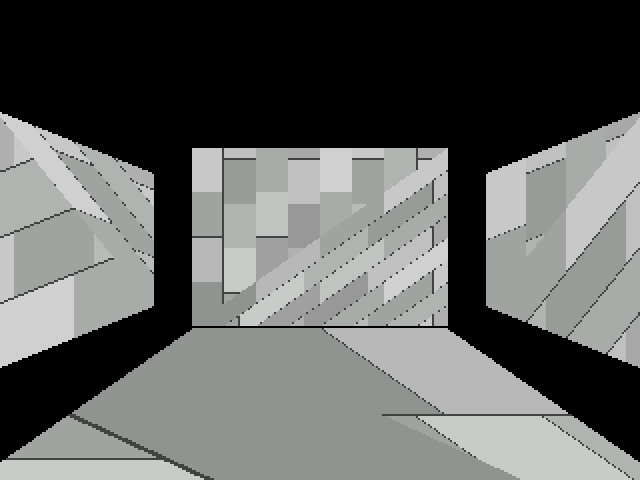
\includegraphics[width=\columnwidth]{orbit_f0.png}\\[2pt]
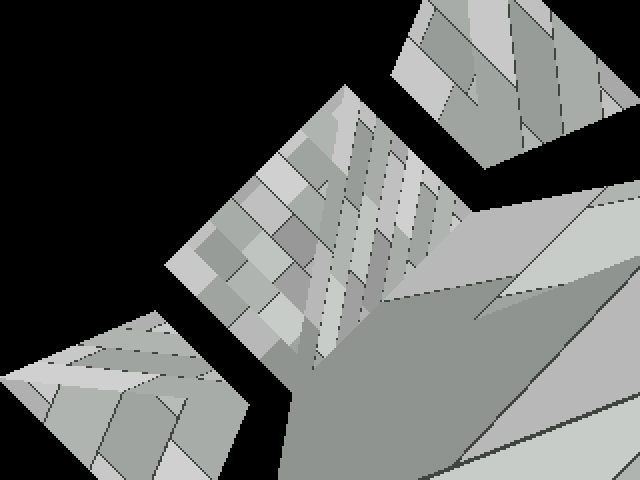
\includegraphics[width=\columnwidth]{orbit_f3.png}
\caption{Orbiting the temple: two frames of a four-frame orbit animation, each
rendered end-to-end through GSX$\to$RTR and verified bit-exact. The scene is
eight textured triangles: back wall, floor and two pillars, using a
procedural brick page.}
\label{fig:orbit}
\end{figure}

\begin{figure}[t]
\centering
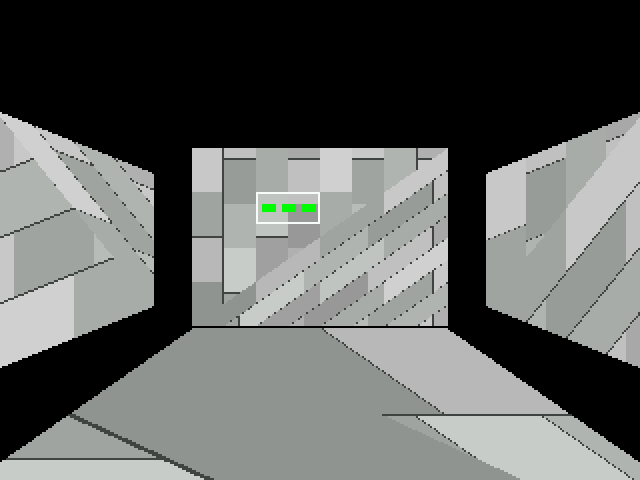
\includegraphics[width=\columnwidth]{fly_f0.png}
\caption{The interactive fly-through: HUD sprite blitted over the temple with
colour-key transparency. Worst frame measured 6.152\,ms, 18.6\% of a 30\,fps
budget at an assumed 100\,MHz; it takes about 12.3\,ms at 50\,MHz.}
\label{fig:fly}
\end{figure}

\begin{figure*}[t]
\centering
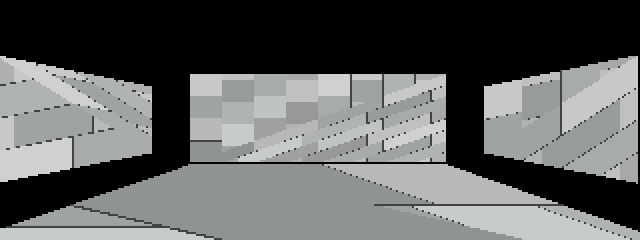
\includegraphics[width=0.24\textwidth]{input_f0.png}\hfill
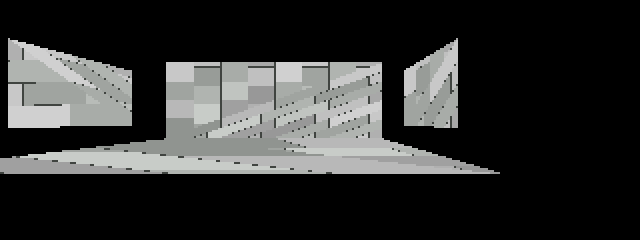
\includegraphics[width=0.24\textwidth]{input_f10.png}\hfill
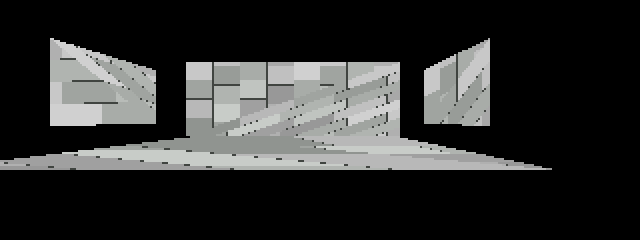
\includegraphics[width=0.24\textwidth]{input_f24.png}\hfill
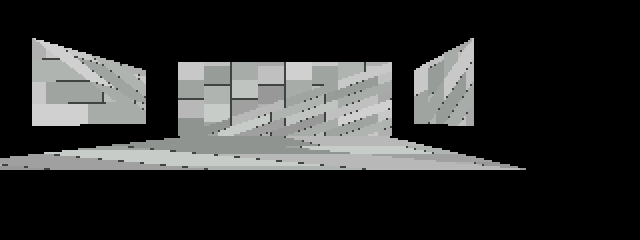
\includegraphics[width=0.24\textwidth]{input_f30.png}
\caption{The input-driven camera walk, frames 0, 10, 24 and 30 of 32. Per-frame
input words are consumed by the game-state kernel on the compute core; the
camera's resulting fp32 position patches the MVP matrix; the scene is then
rendered by the rasterizer. Physics is bit-exact against the golden model on
every frame; 16 of the 32 frames are rasterized to keep simulation time sane.}
\label{fig:input}
\end{figure*}

\subsection{A real level: Doom E1M1}
\label{sec:doom}

A spinning cube proves the pipeline adds up; a real game level proves it is
actually correct, because every wall, flat, light level and texture offset is
someone else's ground truth. \ember{} renders the first level of Doom from the
shareware IWAD (\texttt{data/doom1.wad}) by reading the WAD itself: BSP nodes
and subsectors select the visible segs, sector light levels index the
\textsc{colormap} table for light diminishing, patch-composed wall textures and
64$\times$64 flats are assembled from the WAD's patch directory, and the
vanilla projection is reproduced exactly.

Geometry fidelity comes from emitting Doom's own decomposition instead of
dicing triangles in screen space. Every wall column becomes one quad with $u$
constant and $v$ affine in $y$; every plane row becomes one quad, since a level
camera puts all pixels of a row at a single distance, making $u$ affine in $x$
and $v$ constant. Depth is $1-\mathit{near}/\mathit{dist}$, which is affine in
screen space, so the 16-bit $z$ plane interpolates exactly. The result is
10{,}774 textured triangles in 12 texture-atlas batches, streamed into the real
command queue over the command processor's DMA engine with one 1\,KB palette
load; the rasterizer resolves each texel through that CLUT with the per-triangle
palette bit rather than grey-expanding it.

\begin{figure*}[t]
\centering
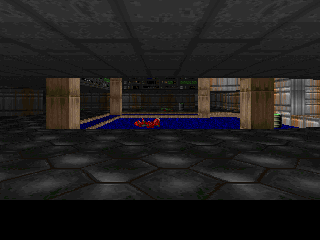
\includegraphics[width=0.32\textwidth]{doom_ref.png}\hfill
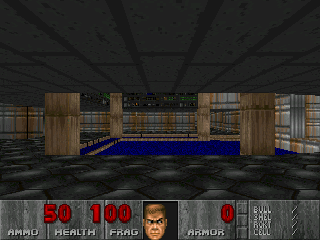
\includegraphics[width=0.32\textwidth]{doom_golden.png}\hfill
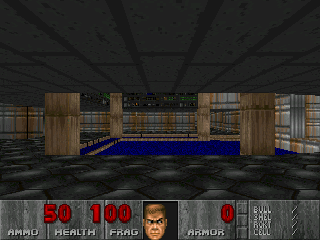
\includegraphics[width=0.32\textwidth]{doom_rtl.png}
\caption{Doom E1M1. (a) the real engine at the player start, for reference;
(b) \ember{}'s golden rasterizer fed 10{,}774 triangles built from the WAD;
(c) the same frame read back out of \texttt{ember\_rtr\_top} in Verilator after
being DMA'd into the command queue. Frames (b) and (c) are identical: 76{,}800
of 76{,}800 pixels, 0 mismatches. 68.4\,ms of simulated time, 232\,s of wall
clock. The reference is letterboxed: Doom renders 320$\times$200, \ember{}
320$\times$240.}
\label{fig:doom}
\end{figure*}

Figure~\ref{fig:doom} is the strongest evidence in this paper that the graphics
pipeline is correct, precisely because no part of the level was designed to
flatter it. The frame out of the RTL is bit-identical to the golden model,
which is itself an independent implementation of Doom's projection and texture
lookup. What is missing is equally clear: sprites, and therefore monsters,
items and the weapon, because sprite patches are transparent-columned and the
rasterizer has no colour-key or alpha path yet; a sprite quad today would be
drawn inside a black box.

\section{Tensor Unit}
\label{sec:tu}

The tensor unit is a 16$\times$16 int8 weight-stationary systolic array with
per-column adder trees, a blocked-$M$ controller and a per-tensor requantization
stage that rounds half-up. It is the AI half of the machine.

Its control logic turned out to be the hard part. Three separate bugs shared one
root cause: counters that were too narrow. Because the array streams full
16-byte tiles, both $K$ and $N$ must be multiples of sixteen; a 4-byte multiple
silently reads the next row's bytes as padding and smears the output
diagonally. Because the controller walks $M$ in blocks, every
``$M$~$\times$~anything'' counter needs enough bits: with a 688-row convolution
output, an 8-bit row counter aliased writes from rows 256--687 back onto rows
0--255, and the square 256-cube test could not possibly catch it.

\subsection{Inference, end to end}

I trained a LeNet-class CNN (conv $1\!\to\!4$ $3\!\times\!3$, pool, conv
$4\!\to\!8$ $3\!\times\!3$, pool, dense $200\!\to\!32\!\to\!10$) in pure Python
with He initialization, a global gradient-norm clip of 400, and an epoch decay
of 0.9, then quantized it to int8 with pure-shift requantization and folded the
biases into the tensor unit's adder taps. Inference runs the image through the
real RTL data path: DMA into VRAM, conv on the tensor unit, pooling as a
kernel on the compute core, conv, pool, dense, dense, with the golden chain
computed in software from the same operands. RTL and software agree
\emph{exactly}, and accuracy is 98/100 = 98.0\% on the first hundred test
images.

\begin{figure}[t]
\centering
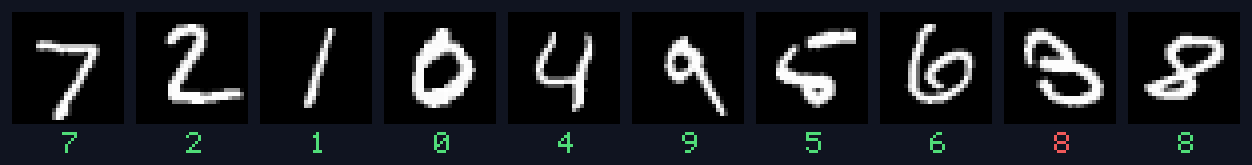
\includegraphics[width=\columnwidth]{mnist_montage.png}
\caption{Ten real MNIST test digits (one per class) with the digit predicted by
the trained int8 model, the same weights the RTL tensor unit executes. Nine
of ten are correct; the miss is a genuinely ambiguous ``3'' that the int8
network calls an ``8''.}
\label{fig:mnist}
\end{figure}

Sustained throughput on a 256$\times$256$\times$256 multiplication is
2{,}134{,}296 cycles. At an assumed 100\,MHz that is \textbf{1.57 GOPS}
sustained against a peak of 51.2 GOPS at the same frequency, about 3.1\%
of peak. At 50\,MHz, both rates halve (0.786 and 25.6 GOPS). This is the
honest cost of the v1 controller: it issues tiles and waits, and the array
spends most of its life streaming operands rather than multiplying. Fixing that
(operand double-buffering and a streaming controller) is the single largest
performance opportunity in the design, and it is deliberately left to the next
revision rather than papered over here.

\section{Verification}
\label{sec:verify}

Every block in this design was verified the same way: write an independent model
in a different language from the RTL, feed both the same stimulus, and require
bit-exact equality. The models live in \texttt{tools/golden/} and are pure
Python, with no numpy, no floats where the hardware is fixed-point, and explicit
modelling of every truncation and rounding step. That last point is what makes
them useful: a golden model that is ``morally'' correct while the RTL truncates
will disagree on a third of the pixels and send you hunting for bugs that do not
exist.

The cocotb suite (Verilator backend) contains 31 tests and passes 31/31. It
covers memory and DMA round trips, bit-exact rasterization including
affine texturing and Z-ordering, the FPU (6{,}720 comparisons, zero
mismatches), the geometry engine, the compute core (including divergence and
barriers), the tensor unit (small multi-tile, quantized, and a 256-cube gate),
MNIST layer by layer and end to end, animation, and the interactive demos. The
Doom bench (Section~\ref{sec:doom}) goes further than the scene demos: it
compares a complete 320$\times$240 level frame against the golden rasterizer,
pixel for pixel, and reports zero mismatches.

\subsection{Verifying a demo with no golden pixels}

Frames that combine a 3D scene with a blitted HUD cannot be compared
pixel-for-pixel against a golden model without reimplementing the whole system
in Python. Instead the demo tests assert \emph{structural} properties that a
broken renderer cannot satisfy: at least twelve distinct colours, at least
20{,}000 non-background pixels, at least fifty distinct depth values, consecutive
frames that differ, and, most importantly, that the HUD's
transparent pixels show the pre-blit scene, which is checked against a snapshot
taken before the blit.

That last check is the kind of thing that sounds paranoid and is not. An earlier
version of this project passed a texture test with a golden model that never
loaded its own checkerboard: golden rendered black, RTL rendered black because
it had lost a single enable bit, and black equalled black for an entire phase.
Since then, every demo test must fail loudly if the golden side is
degenerate.

\subsection{The host interface, without hardware}

The design's host interface is a set of memory-mapped registers, and the
firmware that will run on the NEORV32 is plain C (\texttt{sw/cp\_driver.h},
\texttt{sw/ember\_demo.c}). To prove that interface before owning a board, I
compile the firmware as a normal translation unit against a Verilator harness
that implements a cycle-accurate AXI4-Lite master, and run it against the full
top level. The demo executes all 32 frames, uploads textures, launches kernels,
polls completion cookies, drives the geometry engine and the rasterizer, and
draws its final frame. That frame matches the cocotb testbench's frame 30 on
\textbf{10{,}316 of 10{,}316} scene pixels. The firmware that will ship is the
firmware that was tested.

\section{ASIC Implementation}
\label{sec:asic}

\begin{figure}[t]
\centering
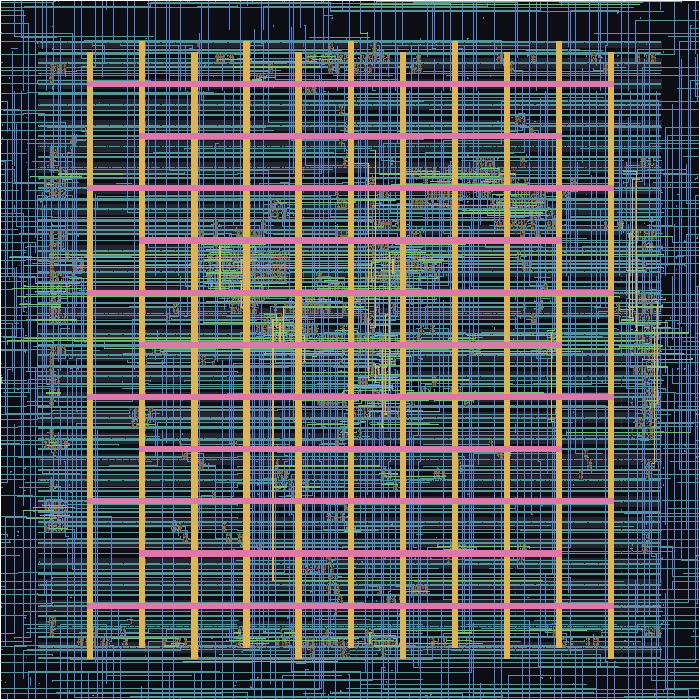
\includegraphics[width=\columnwidth]{gds_block.png}
\caption{Actual crossbar block layout rendered from independently audited
GDS-II: 182.5$\times$182.5\,$\mu$m. Routing and whole-layout Magic DRC report
zero errors. This is an individual block, not an integrated GPU die.}
\label{fig:die}
\end{figure}

The logical design is only half of a GPU. The other half is geometry: polygons,
wells, routes, and a GDS-II file that a foundry could, in principle, accept.
I run a custom block-level flow inside the OpenLane~2 tool container.
Using that container does not mean the complete OpenLane sign-off flow has
been executed. The block implementation stages are:

\begin{enumerate}
  \item \textbf{SystemVerilog $\to$ Verilog-2005} with \texttt{sv2v}. My RTL
        uses packages and packed structs, which Yosys's built-in frontend
        rejects; \texttt{sv2v} inlines packages and lowers structs to vectors,
        giving clean Verilog-2005 that any tool can read.
  \item \textbf{Logic synthesis} with Yosys~0.46 and ABC, targeting the
        sky130 high-density standard-cell library, with the
        \texttt{sky130\_fd\_sc\_hd\_\_tt\_025C\_1v80} corner.
  \item \textbf{Floorplan, placement, clock tree and routing} with OpenROAD:
        20--30\% target utilization, routability-driven global placement,
        repair plus detailed placement, CTS, RC estimation and detailed routing.
  \item \textbf{DRC and GDS export} with Magic, then final GDS normalization
        with KLayout.
\end{enumerate}

\begin{figure}[t]
\centering
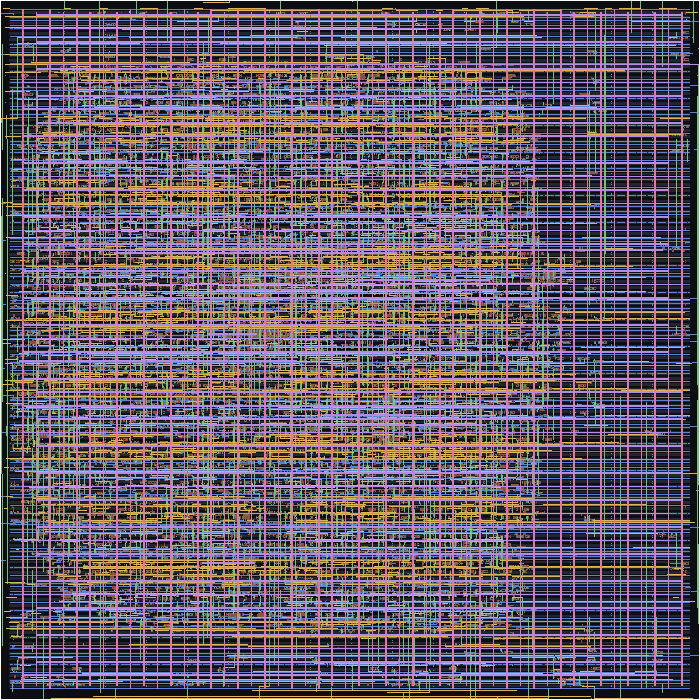
\includegraphics[width=\columnwidth]{gds_cp.png}
\caption{Actual command-processor exported layout, 706.475$\times$706.475\,$\mu$m
on sky130. Detailed routing and the independent whole-layout Magic audit
both report zero violations. Colour denotes physical layer; LVS and timing
sign-off remain pending.}
\label{fig:gds}
\end{figure}

Table~\ref{tab:asic} lists the twelve blocks (rasterizer scan and setup, the
full rasterizer top, the vector FPU, the geometry engine, the blitter, display,
command processor, crossbar, register-file slave, compute core and tensor unit)
with cell counts, design area, routed wire length, worst negative slack against
a 20\,ns target clock, DRC count and GDS size.

Two synthesis issues required explicit corrections. Behavioral processes must
be lowered before custom technology mapping; a successful tool exit alone did
not prove a fully mapped netlist. I validate the exported JSON netlist for
residual processes and generic cells. The multiplier-heavy raster scan unit
also exceeded available memory during ABC mapping. A reduced mapping script
and ripple-carry arithmetic mapping produced a validated netlist, but not a
completed physical layout. These are implementation experiments, not evidence
of timing closure.

\subsection{Integrated-die implementation status}

I have prepared an integration candidate containing eight top-level logic
macros: crossbar, command processor, tensor unit, compute core, geometry
engine, blitter, rasterizer top and display. The vector FPU, register slave,
and raster setup and scan occur within parent blocks; placing all twelve
standalone targets on a die would duplicate functionality. The candidate's
synthesized wrapper contains 261 cells in total, including eight macro
instances and 253 standard cells. Corrected accelerator memory-port wiring
is included in this netlist.

This candidate exposes VRAM-facing interfaces at die ports. It is an
external-memory logic variant, not a physical implementation of the original
512\,KB on-chip-memory GPU. A compatible memory implementation, macro
interface checks, power connectivity, inter-block routing, full-die DRC, LVS
and extracted timing remain necessary. No integrated-die GDS has been completed
or independently audited. Figure~\ref{fig:die} therefore shows an actual
verified block, not a full chip.

% generated by tools/gds/collect_results.py (complete table float)
% AUTO-GENERATED by tools/gds/collect_results.py: do not edit
\begin{table}[t]
\caption{SkyWater sky130 hardening results, per block. Cells are mapped standard cells after synthesis (hierarchical wrappers include macro instances); area and wire length are from the latest available physical run; DRC is the exported-layout audit count when verified, otherwise the available Magic count; missing entries are not completed results. WNS is worst negative slack against a 20\,ns (50\,MHz) target.}
\label{tab:asic}
\centering
\scriptsize
\begin{tabular}{@{}lrrrrrr@{}}
\toprule
Block & Cells & Area & Wire & WNS & DRC & GDS \\
      &       & ($\mu m^2$) & ($\mu m$) & (ns) & & (KB) \\
\midrule
\texttt{rtr\_scan} & 1416166 & - & - & - & - & - \\
\texttt{rtr\_setup} & 20782 & 150387 & 853284 & 0.00 & 0 & 57106 \\
\texttt{rtr\_top} & - & - & - & - & - & - \\
\texttt{fpu4} & 101131 & 712822 & 3665444 & -48.87 & - & 38284 \\
\texttt{gsx} & 113334 & - & - & - & - & - \\
\texttt{blit} & 2169 & 22326 & 81022 & 0.00 & 0 & 8652 \\
\texttt{display} & 454 & 6061 & 16149 & 0.00 & 0 & 2100 \\
\texttt{cp} & 7593 & 119186 & 568455 & 0.00 & 0 & 40451 \\
\texttt{xbar} & 267 & 3187 & 68220 & 0.00 & 0 & 2571 \\
\texttt{ram\_slave} & 158 & 5573 & 22661 & 0.00 & 0 & 1850 \\
\texttt{core} & 347494 & - & - & - & - & - \\
\texttt{tu} & 257363 & - & - & - & - & - \\
\bottomrule
\end{tabular}
\end{table}


\section{Results}
\label{sec:results}

\subsection{Graphics}

The rasterizer is a multi-cycle FSM, not a one-pixel-per-clock pipeline.
The worst frame of the interactive
fly-through (eight textured triangles plus a keyed HUD sprite over 320$\times$240)
takes 613{,}000 cycles in the rasterizer and 2{,}067 cycles in the blitter:
\textbf{6.152\,ms at an assumed 100\,MHz, or 12.303\,ms at 50\,MHz}.
These occupy about 18.5\% and 36.9\% of a 33.3\,ms budget, respectively. The
orbit animation and the input-driven walk show the same order of magnitude. That
is a cycle-based simulation estimate, not an achieved silicon clock rate.

\begin{figure}[t]
\centering
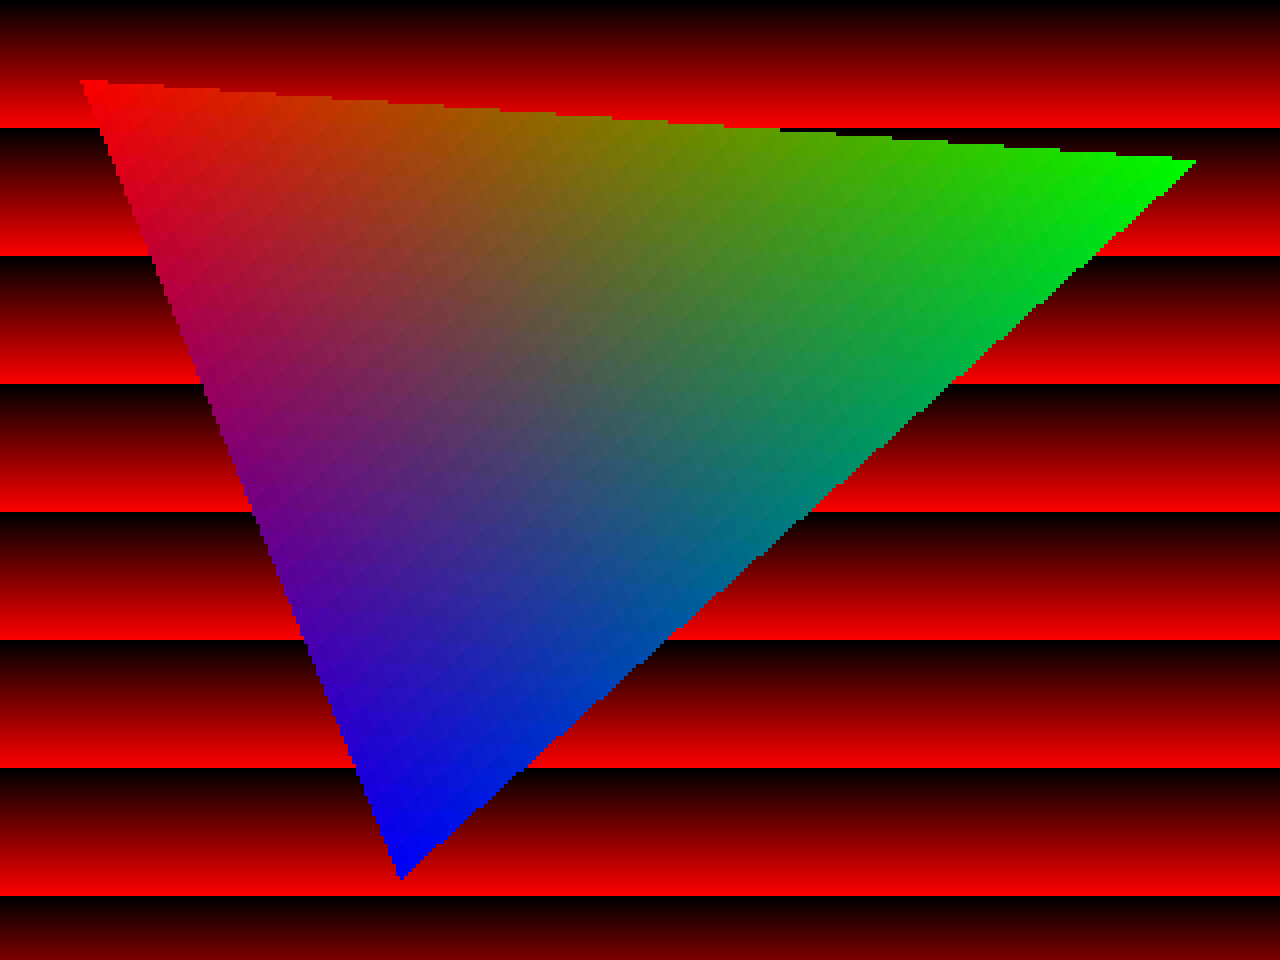
\includegraphics[width=\columnwidth]{display_frame.png}
\caption{Composite frame captured from the display pipeline: rasterized
triangle over a gradient, doubled to 640$\times$480 by the display's
double-scan path.}
\label{fig:display}
\end{figure}

\subsection{Inference}

98.0\% accuracy on the first hundred MNIST test images, through the real RTL
data path, with the software mirror agreeing exactly. Sustained tensor
throughput is 1.57 GOPS at 100\,MHz in this revision.

\subsection{Sim-to-silicon}

Table~\ref{tab:asic} reports the current per-block evidence, not a completed
chip. \AsicBlocksGds{} blocks (crossbar, display, register slave, blitter,
command processor and raster setup) have exported GDS independently checked by reimporting and flattening the placed design in
Magic with all rules enabled. Tapless library masters fail well-tap checks in
isolation, so those checks require the assembled context with neighbouring tap
cells. The generated table records \AsicBlocksDone{} completed synthesis targets.
Raster setup and scan have mapped-netlist evidence; the rasterizer top
currently has a glue netlist with blackboxed setup and scan, not a completed
physical macro. An earlier zero-exit synthesis run was rejected because ABC
skipped modules containing processes. Physical builds of the remaining targets are in progress. No LVS pass, timing closure,
pad ring, implemented 512\,KB SRAM or electrically routed chip assembly is
claimed. Parent and child targets overlap and their cell counts must not be
summed as the area of a single GPU.

\section{What Went Wrong, and What It Taught Me}
\label{sec:lessons}

The following are the bugs that cost the most time. I list them because they
generalize far beyond this project.

\textbf{A single shared instruction buffer makes barriers deadlock.} Thread~0
reaches the barrier first; its next fetched instruction wedges the only buffer;
the buffer never frees; threads 1--3 never execute. The fix, per-thread
one-word buffers, looks obvious \emph{after} you have spent a day staring at a
core that looks perfectly alive and makes no progress.

\textbf{Fetch and load must not share a port.} The same circular wait, one level
down: a thread waiting on a load holds the instruction buffer while the fetch
that would unblock it cannot get the memory port. Separate ports fix it.

\textbf{Only one instruction sets the flags.} In this ISA, \texttt{CMP} sets
neg/zero/pos and every other ALU operation is flag-silent. A kernel that
subtracts and then branches on the result simply never loops, and it looks
like a hang, not like a logic error.

\textbf{Branch condition letters name the flags tested, not the meaning.}
\texttt{BRNZP nz} branches when \emph{negative or zero}, not ``if not zero''. A
three-way sign split written that way silently took the wrong path; two
branches in my physics kernel had to become single-flag branches.

\textbf{Logical shifts bite signed values.} Computing friction as
\texttt{(K*v) >> 16} is a catastrophe for negative velocities, because the shift
is logical: a negative product becomes a huge positive number and slams the
velocity into the clamp. The fix is magnitude-plus-sign, not arithmetic, and the
golden model must reproduce the branch exactly.

\textbf{Wide counters are a correctness requirement, not a detail.} The tensor
unit's $M$ counter at 8 bits aliased 688 output rows onto 256; the square
256-cube test could not fail. Test non-square shapes even when the flagship gate
test is square.

\textbf{Reading a result the same cycle you request it, races.} The FPU's
busy-poll protocol occasionally sampled a stale zero. Fixed-latency interfaces
are easier to verify than free-running ones; where I could not use fixed
latency I had to define, precisely, which cycle a value is valid.

\textbf{Memory layouts hide bugs better than logic does.} Two of the worst
week-long bugs in this project were stride errors: a row stride reused for a
column stride (invisible when $K=N$) and an op-major tensor output consumed as
plane-major (which scrambles channels silently). Both were only caught by
comparing intermediate values, layer by layer, rather than final results.

\textbf{A test can pass for the wrong reason, and that is the dangerous case.}
Black equalled black through a whole phase. My response was structural: every
demo test now asserts properties that a degenerate renderer cannot satisfy.

\textbf{Simulation time is a design constraint.} Keeping 32 frames inside one
foreground run forced me to sample the framebuffer rather than dump it, to
render every other frame while advancing physics every frame, and to find out the
hard way that skipping the framebuffer clear leaves stale pixels piled into
sawtooth ``mountains'' that lower-bound assertions cannot detect.

\section{Availability and Reproducibility}

Everything is in one repository: RTL, golden models, assembler, kernels, cocotb
tests, the bare-metal C driver and demo, the Verilator host harness, the layout
scripts and this paper's sources. The only external requirements are
Verilator, cocotb, Yosys, OpenROAD, Magic, KLayout, \texttt{sv2v} and a
sky130 PDK, all open source. \texttt{make lint} and \texttt{cd test \&\& make}
reproduce the verification results; \texttt{scripts/gds/run\_all.sh} reproduces
the layout flow.

\section{Conclusion}

Building a GPU from scratch is a good way to learn how much of computer
architecture is about interaction rather than invention. The multiplier array,
the rasterizer FSM and the crossbar are each textbook objects; almost every
hour of debugging in this project went into the interfaces between them:
who owns the memory port, who sets the flags, which counter is wide enough,
which buffer can block whose progress. \ember{} now runs a real neural network
at 98\% accuracy on the 100-image evaluation subset, a simulated 3D game
loop, and several DRC-checked routed block layouts on an open process. Those results address the goal I set. In the spirit of the lessons
section, I am clear about what it is not: not
fast, not manufacturable without sign-off work, and not the last revision.

\section*{Acknowledgment}
All EDA tools used here are open source, and every result in this paper was
produced on a single Windows/WSL machine. Earlier synthesis runs used a
21\,GB WSL allocation; current physical builds run with a 16\,GB cap. Thanks
to the maintainers of Verilator, cocotb, Yosys, OpenROAD, Magic, KLayout and the
sky130 PDK.

\begin{thebibliography}{99}
\bibitem{tpu} N.~Jouppi \emph{et al.}, ``In-datacenter performance analysis of a
tensor processing unit,'' \emph{ISCA}, 2017.
\bibitem{kung} H.~T.~Kung and C.~E.~Leiserson, ``Systolic arrays for VLSI,''
\emph{Sparse Matrix Proceedings}, 1978.
\bibitem{miaow} N.~K.~Vedula \emph{et al.}, ``MIAOW: An open source GPGPU,''
\emph{ISCA}, 2014.
\bibitem{vortex} B.~Tine \emph{et al.}, ``Vortex: Extending the RISC-V ISA for
GPGPU,'' \emph{MICRO}, 2017.
\bibitem{nyuzi} J.~Bush \emph{et al.}, ``Nyuzi: A GPGPU processor,''
open-source project.
\bibitem{gemmini} H.~Genc \emph{et al.}, ``Gemmini: Enabling systematic deep
learning architecture evaluation,'' \emph{MICRO}, 2021.
\bibitem{verilator} W.~Snyder, ``Verilator,'' open-source project.
\bibitem{cocotb} Cocotb contributors, ``cocotb: a coroutine-based testbench
framework,'' open-source project.
\bibitem{neorv32} S.~Noltmann, ``NEORV32: an open-source RISC-V soft core,''
open-source project.
\bibitem{sky130} SkyWater Technology and Google, ``SkyWater 130\,nm open PDK.''
\bibitem{openlane} Efabless, ``OpenLane 2: an open-source ASIC flow,''
open-source project.
\bibitem{openroad} The OpenROAD Project, ``OpenROAD: toward a
self-driving, open-source digital layout implementation tool chain.''
\bibitem{sv2v} Z.~Smith, ``sv2v: SystemVerilog to Verilog conversion,''
open-source project.
\end{thebibliography}

\end{document}
